
\section{Literature Review}

\subsection{Normal Determination}
	For a point to exist in a cloud and have x, y, z colour and intensity values associated with it, the point will have had to be on the surface of something. So with this knowledge we can start to create information about this point.
	
	\subsubsection{Principal Components Analysis}
	Principal Components Analysis (PCA), is a statistical technique that transforms a number of possibly correlated variables into a smaller number of uncorrelated variables called Principal components. the number of principal components is less than or equal to the dimensions of the data set, so in the case of point clouds 3.
	
	The first of the Principal components represents the largest variability in the data set, with the variability decreasing as you go along. essentially resulting in the 3rd Principal component being the normal to the surface \citep{dunteman_principal_1989}. 
	
	\subsubsection{Plane fitting}
		you fit planes to it and thats that.
	

	
\subsection{Segmentation}
	For automatic processing of point clouds the segmentation of the point cloud is one of the most important processes. it is important that the segmentation of the point cloud is correct and the method is the best for the use.

	\subsubsection{Edge-based Segmentation}
		Edge-based segmentation has two main sections to it; first to detect edges in the point cloud, and secondly to group all points contained within the edges as one segment.
		
		The algorithm used, however, does not use Edge-based techniques further reading on the topic can be found with \cite{sappa_fast_2001} and \cite{bhanu_automatic_1986}.
		
		
	\subsubsection{Region-based Segmentation}
		Region-based segmentation algorithms look for areas that fit into a certain criteria and group them together as a single region.
		
		Region growing for 3D point clouds is an adapted algorithm that was originally created by \cite{adams_seeded_1994} for the segmentation of intensity images.
		
		Region growing needs two things; first, seed points based on their curvature values, and secondly criteria in which to extend these points into regions.
		
		There are several methods for doing these two things as described by \cite{hoover_experimental_1996}.
		
		Point Cloud Libraries region growing algorithm starts off by calculating the curvature for each point then sorting all points by their curvature value. this is because the point with the least curvature associated with it is located in the flattest section of the point cloud. Once the cloud is sorted the region growing part of the algorithm begins:

		\renewcommand\labelitemi{{\boldmath$\cdot$}}
		\begin{itemize}
			\item The algorithm picks the point with the smallest curvature and adds it to a set called seeds.
			
			\item For every seed point the algorithm looks at all the neighbors and decides if they are part of that seeds region or not. This is done by looking at certain criteria with user specified thresholds.
			
			\begin{itemize}
				\item Does the points normal deviate by more than the user specified threshold from the seed point.
				
				\item Does the points curvature deviate by more than the user specified threshold from the seed point.
				
			\end{itemize}
			
			\item Once no more points are found for that particular seed, or the region reached a specified maximum, the seed is removed from the set of seeds and the region as added to the global segment list. If no more seeds are in the set the process is started from the beginning again, except this time the points that have been assigned to a region are no longer available to be seed points or to become part of a region.
			
		\end{itemize}
		
		If after a seed point has been through the process and the number of points does not reach the user defined minimum size the whole region removed from the cloud as unclassified and will inevitably be removed by the user.
		
		
		\begin{figure}[H]
			\centering
			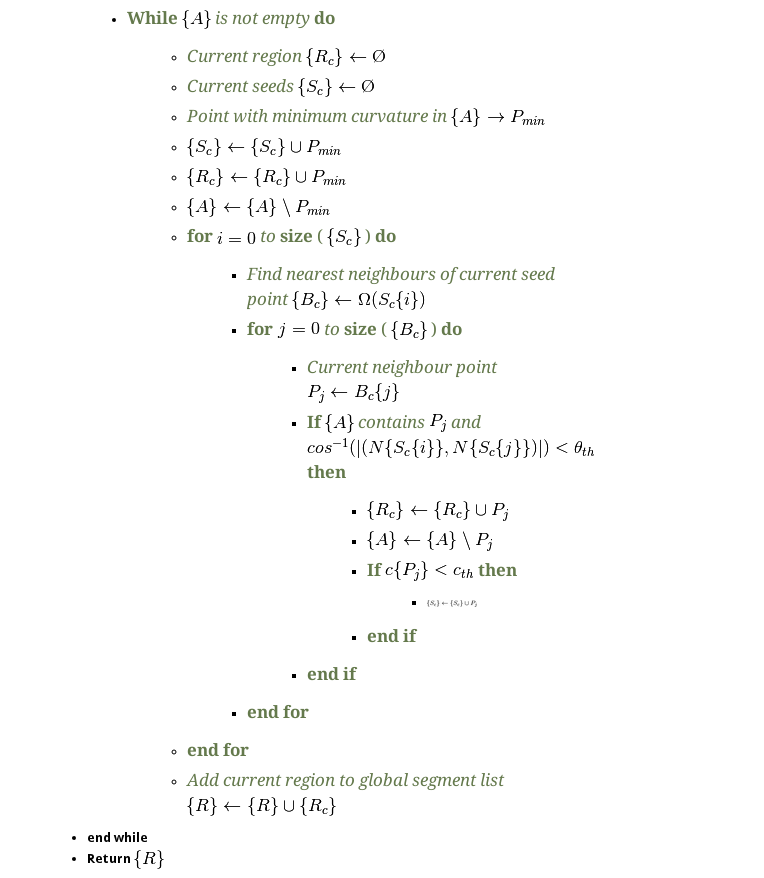
\includegraphics[width=0.7\linewidth]{Includes/images/LitReview/RegionGrowing}
			\caption{Pseudo code for region growing algorithm}
			\label{fig:RegionGrowing}
		\end{figure}

		

\subsection{Open Multi-Processing}
	OpenMP is an application programming interface (API) for writing multi-threaded applications. Certain functions in Point Cloud Library have support for multi-threading using OpenMP.
		

		
		
		
		
		
		
		
		
		
		